\documentclass[final,t]{beamer}
\mode<presentation>
{
%  \usetheme{Warsaw}
%  \usetheme{Aachen}
%  \usetheme{Oldi6}
%  \usetheme{I6td}
  \usetheme{I6dv}
%  \usetheme{I6pd}
%  \usetheme{I6pd2}
}
% additional settings
\setbeamerfont{itemize}{size=\normalsize}
\setbeamerfont{itemize/enumerate body}{size=\normalsize}
\setbeamerfont{itemize/enumerate subbody}{size=\normalsize}
% additional packages
\usepackage{ragged2e}
\usepackage{verbatim}
\usepackage{textcomp}
\usepackage[ampersand]{easylist}
\usepackage{lipsum}
\usepackage{times}
\usepackage{amsmath,amsthm, amssymb, latexsym}
\usepackage{exscale}
%\boldmath
\usepackage{booktabs, array}
%\usepackage{rotating} %sideways environment
\usepackage[english]{babel}
\usepackage[latin1]{inputenc}
\usepackage[orientation=landscape,size=custom,width=109.728,height=88.9,scale=1]{beamerposter}
\addtobeamertemplate{block begin}{}{\justifying}
\listfiles
\graphicspath{{figures/}}
% Display a grid to help align images
%\beamertemplategridbackground[1cm]

\title{\huge scikit-bio: a Python library for bioinformaticians and data scientists}
\author{Evan T. Bolyen$^{a,b}$, The scikit-bio Development Team$^{c}$ and J. Gregory Caporaso$^{a,b,d}$}
\institute{$^{a}$Center for Microbial Genetics and Genomics - Northern Arizona Univ.; $^{b}$Department of Computer Science - Northern Arizona Univ.;\\ $^{c}$https://github.com/biocore/scikit-bio/graphs/contributors; $^{d}$Department of Biological Sciences - Northern Arizona Univ.}

% abbreviations
\usepackage{xspace}
\makeatletter
\DeclareRobustCommand\onedot{\futurelet\@let@token\@onedot}
\def\@onedot{\ifx\@let@token.\else.\null\fi\xspace}
\def\eg{{e.g}\onedot} \def\Eg{{E.g}\onedot}
\def\ie{{i.e}\onedot} \def\Ie{{I.e}\onedot}
\def\cf{{c.f}\onedot} \def\Cf{{C.f}\onedot}
\def\etc{{etc}\onedot}
\def\vs{{vs}\onedot}
\def\wrt{w.r.t\onedot}
\def\dof{d.o.f\onedot}
\def\etal{{et al}\onedot}
\makeatother

%%%%%%%%%%%%%%%%%%%%%%%%%%%%%%%%%%%%%%%%%%%%%%%%%%%%%%%%%%%%%%%%%%%%%%%%%%%%%%%%%%%%%%%%%%%%%%%%%%%%%%%%%%%%
%%%%%%%%%%%%%%%%%%%%%%%%%%%%%%%%%%%%%%%%%%%%%%%%%%%%%%%%%%%%%%%%%%%%%%%%%%%%%%%%%%%%%%%%%%%%%%%%%%%%%%%%%%%%
\begin{document}
\begin{frame}{}
  \begin{columns}[t]
    \begin{column}{.3\linewidth}
        \begin{alertblock}{
\includegraphics[width=1\linewidth]{assets/skbio}\newline\newline}
          scikit-bio is an open-source, BSD-licensed Python package providing data structures, algorithms and educational resources for bioinformatics.
          \newline
        \end{alertblock}

        \begin{block}{GOALS}
            \begin{itemize} {\fontsize{32pt}{40pt}
                \item[$\bullet$] \textbf{Simple to use}
                \item[$\bullet$] \textbf{Make building tools like QIIME $^{[1]}$ easier}
                \item[$\bullet$] \textbf{Extensive supporting documentation}
                \item[$\bullet$] \textbf{Domain specific API that maps biological vocabulary to implementation}
                \item[$\bullet$] \textbf{Optimized wherever possible}
                \item[$\bullet$] \textbf{Rigorously tested}
                }
            \end{itemize}
        \end{block}

        \begin{block}{Intended Audience}
            \textbf{Features for Biology Students:}
            \begin{itemize}
                \item[$\bullet$]Excellent documentation
                \item[$\bullet$]External resources
                \item[$\bullet$]Easy to understand error messages
            \end{itemize}
            \vspace{1cm}
            \textbf{Features for Bioinformatics Developers:}
            \begin{itemize}
                \item[$\bullet$]Rigorously tested optimizations
                \item[$\bullet$]File format and external library interoperability
                \item[$\bullet$]Performance ``escape-hatches''
            \end{itemize}
            \vspace{1cm}
            \textbf{Features for Data Scientists:}
            \begin{itemize}
                \item[$\bullet$]Powerful integration with IPython $^{[2]}$ (Jupyter) notebooks
                \item[$\bullet$]Data validation
                \item[$\bullet$]Consistent API
            \end{itemize}
        \end{block}


        \begin{block}{Projects Using scikit-bio}
            \textbf{Current Projects:} \\
            \begin{itemize}{\fontsize{28pt}{36pt}
              \item[$\bullet$] QIIME 1.9 $^{[1]}$ - Quantitative Insights Into Microbial Ecology \hfill \\
              Used as the core library that powers most of the scripts available.
              \newline
              \item[$\bullet$] ghost-tree $^{[3]}$ - 18S/ITS Phylogenetic Scaffolding System \hfill \\
              Uses IO and TreeNode to read databases and manipulate phylogenies to produce a combined 18S/ITS tree.
              \newline
              \item[$\bullet$] Qiita $^{[4]}$ - Spot Patterns \hfill \\
              Uses many aspects of scikit-bio (and QIIME) to analyze -omics data.
              \newline
              }
            \end{itemize}

            \textbf{Future Projects:} \\
            \begin{itemize}{\fontsize{28pt}{36pt}
              \item[$\bullet$] QIIME 2 - A stronger, faster, easier to use QIIME \hfill \\
              Still under development, but scikit-bio will be used by the entirety of this project.
              \newline}
          \end{itemize}
        \end{block}

      %%%%%%%%%%%%%%%%%%%%%%%%%%%%%%%%%%%%%%%%%%%%%%%%%%%%%%%%%%%%%%%%%%%%%%%%%%%%%%%%%%%%%%%%%%%%%%%%%%%%%%%%%%%%


    \end{column}
    \begin{column}{.3\linewidth}
        %%%%%%%%%%%%%%%%%%%%%%%%%%%%%%%%%%%%%%%%%%%%%%%%%%%%%%%%%%%%%%%%%%%%%%%%%%%%%%%%%%%%%%%%%%%%%%%%%%%%%%%%%%%%



        \begin{block}{Use Case: Identify File Formats}
            One of the exciting features of scikit-bio are ``sniffers'' which can automatically detect the format of a file so that it can be read into a data-structure. \newline\newline
            \python{assets/py/sniff.py}
            \verbatiminput{assets/sniff.out} \vspace{1cm}
            This step is automatically done in all of scikit-bio's IO methods.
        \end{block}

        \begin{block}{Use Case: Simple Query Mapping}
          We can define a simple function for this purpose. (We compute a global alignment and find the Hamming distance between the aligned sequences).
          \newline\newline
          \python{assets/py/pairwise_similarity.py}
          \verbatiminput{assets/pairwise.out}
        \end{block}

        \begin{block}{Use Case: Biological Diversity Analysis}
            With scikit-bio it is possible to reach the same conclusions as Lauber CL et al. 2009 $^{[5]}$ from within an IPython $^{[2]}$ (Jupyter) notebook. To see the entire replicated study, see ``Exploring microbial community diversity'' in the scikit-bio ``cookbook''.
            \newline\newline
            \python{assets/py/pcoa.py}
            \centerline{\includegraphics[width=.6\linewidth]{assets/ordination_out.eps}}\\
        \end{block}


    \end{column}

    %%%%%%%%%%%%%%%%%%%%%%%%%%%%%%%

    \begin{column}{.3\linewidth}
        \begin{block}{Documentation}
            Documentation for scikit-bio is available in many forms:
            \begin{columns}
                \begin{column}{.45\linewidth}
                    \begin{minipage}[c][20cm][c]{\linewidth}
                        \href{http://scikit-bio.org}{\color{blue}\underline{scikit-bio.org}}
                        \newline\newline
                        Our website provides\\ \textbf{complete} API documentation. Included are: inputs, outputs, reference material, and examples. In addition we provide the scikit-bio ``cookbook'' which has even more in-depth examples and use-cases (\href{http://scikit-bio.org/cookbook}{\color{blue}\underline{scikit-bio.org/cookbook}}).

                    \end{minipage}
                    \begin{minipage}[c][15cm][c]{\linewidth}
                        \href{http://applied-bioinformatics.org}{\color{blue}\underline{applied-bioinformatics.org}}
                        \newline\newline
                        Introduction to Applied Bioinformatics is a companion, open source, interactive text that teaches bioinformatics concepts and techniques using scikit-bio.
                    \end{minipage}
                \end{column}
                \begin{column}{.45\linewidth}
                    \begin{minipage}[c][20cm][c]{\linewidth}
                        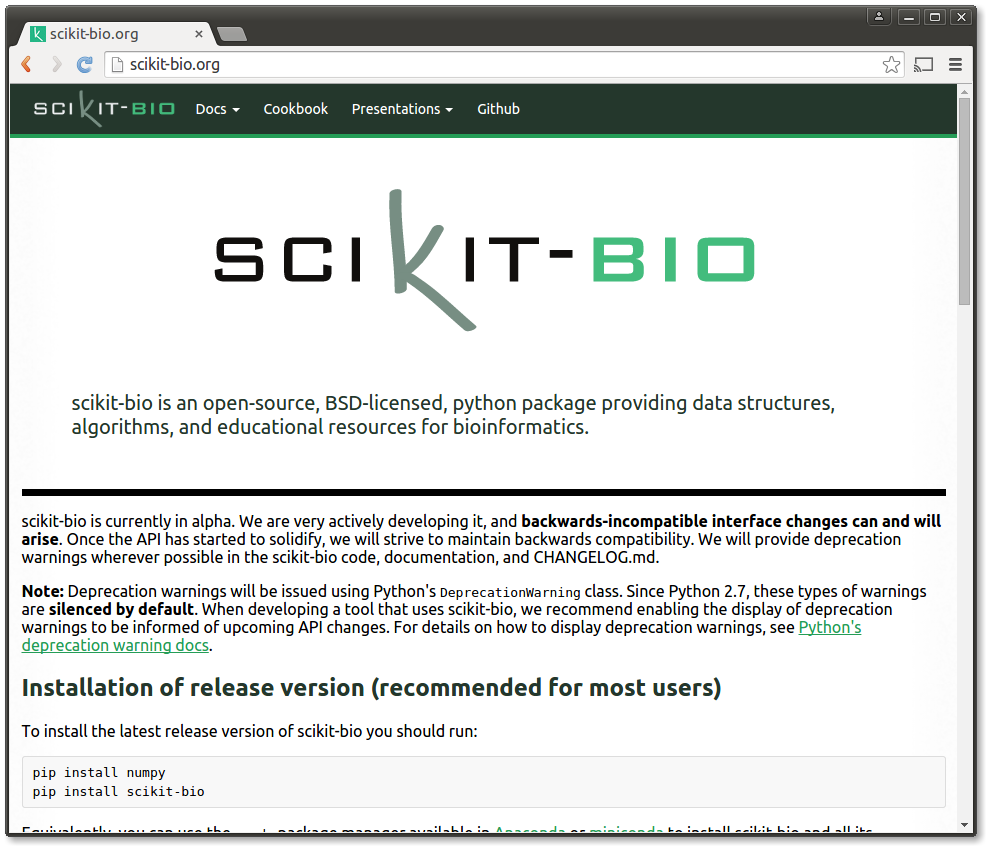
\includegraphics[width=1\linewidth]{assets/website}\\
                    \end{minipage}
                    \begin{minipage}[c][15cm][c]{\linewidth}
                        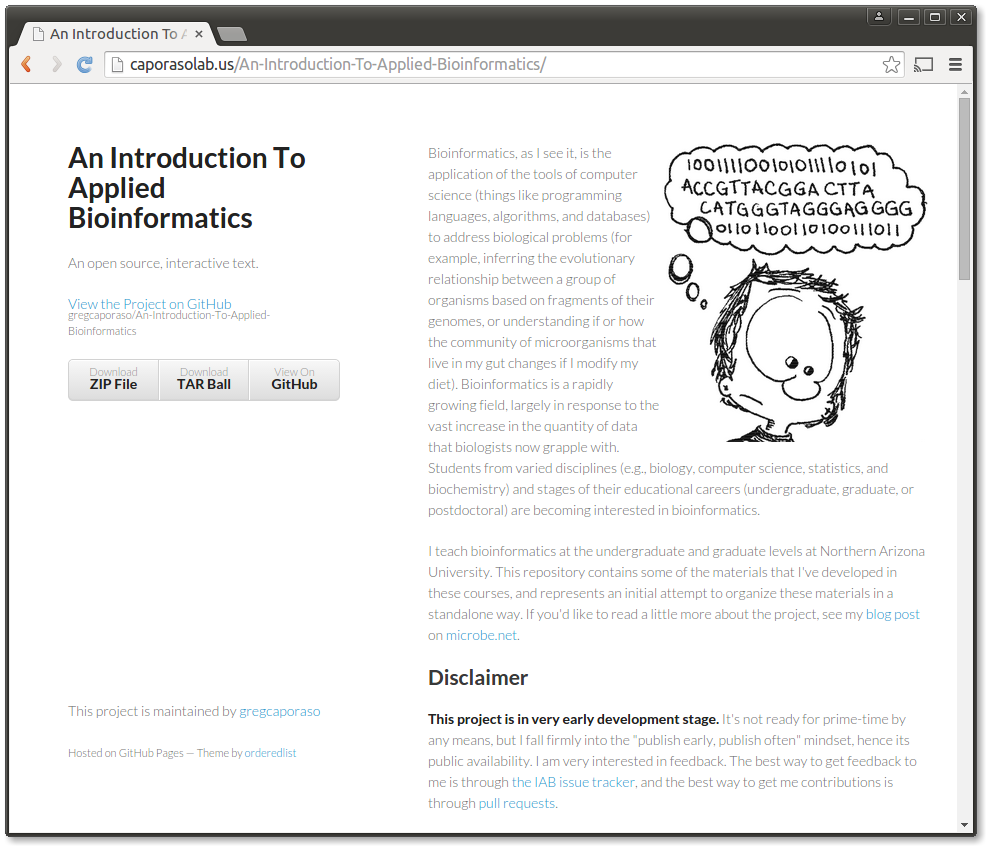
\includegraphics[width=1\linewidth]{assets/iab}\\
                    \end{minipage}
                \end{column}
            \end{columns}
            Additionally, all API documentation is accessible from within the source code, an interactive session, and IPython $^{[2]}$ (Jupyter).

        \end{block}



        \begin{block}{Future Work}
            There is still a lot of work to do. We are currently working through our entire API and normalizing the vocabulary and behavior. Additionally we plan to add many more file formats.
            We intend to have a beta-release and a paper publication in conjunction with the SciPy 2015 conference (beginning of July).

        \end{block}
        \begin{block}{References}
            \begin{itemize}
              {\small
              \item[1]Caporaso, J Gregory et al. ``QIIME allows analysis of high-throughput community sequencing data.'' Nature methods 7.5 (2010): 335-336.
              \item[2]Perez, Fernando, and Brian E. Granger. ``IPython: a system for interactive scientific computing.'' Computing in Science \& Engineering 9.3 (2007): 21-29.
              \item[3]Fouquier, Jennifer et al. ``ghost-tree: a tool for creating fungal hybrid-gene phylogenetic trees.'' Manuscript in preparation.
              \item[4]http://qiita.microbio.me
              \item[5]Lauber, Christian L., et al. ``Pyrosequencing-based assessment of soil pH as a predictor of soil bacterial community structure at the continental scale.'' Applied and environmental microbiology 75.15 (2009): 5111-5120.
              }
          \end{itemize}
        \end{block}

        %%%%%%%%%%%%%%%%%%%%%%%%%%%%%%%%%%%%%%%%%%%%%%%%%%%%%%%%%%%%%%%%%%%%%%%%%%%%%%%%%%%%%%%%%%%%%%%%%%%%%%%%%%%%



%%%%%%%%%%%%%%%%%%%%%%%%%%%%%%%%%%%%%%%%%%%%%%%%%%%%%%%

    \end{column}
  \end{columns}

\end{frame}

\end{document}


%%%%%%%%%%%%%%%%%%%%%%%%%%%%%%%%%%%%%%%%%%%%%%%%%%%%%%%%%%%%%%%%%%%%%%%%%%%%%%%%%%%%%%%%%%%%%%%%%%%%
%%% Local Variables:
%%% mode: latex
%%% TeX-PDF-mode: t
%%% End:
